\autobookmark
\begin{frame}[t]{Adaptive sampling to counter high MSE values}
      \myonly{1}{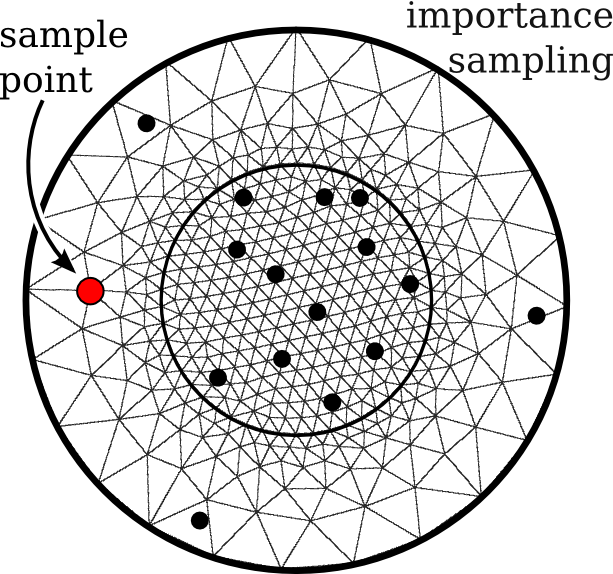
\includegraphics[width=.37\paperwidth]{graphics/ray_distributions3.png}}
      \myonly{2}{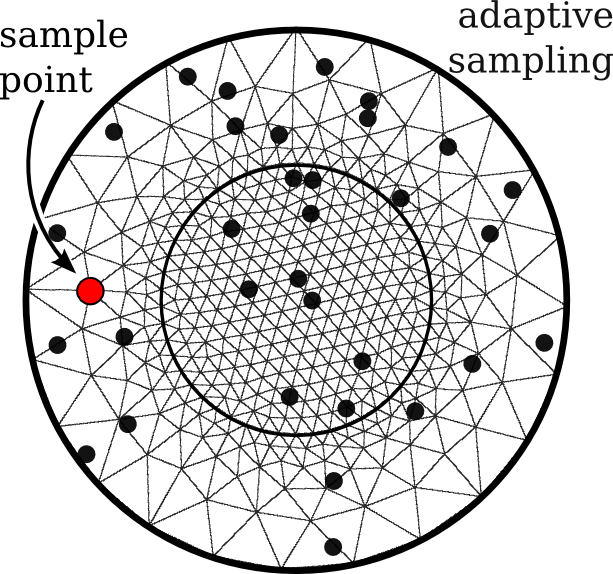
\includegraphics[width=.37\paperwidth]{graphics/ray_distributions4.png}}
      \myonly{1}{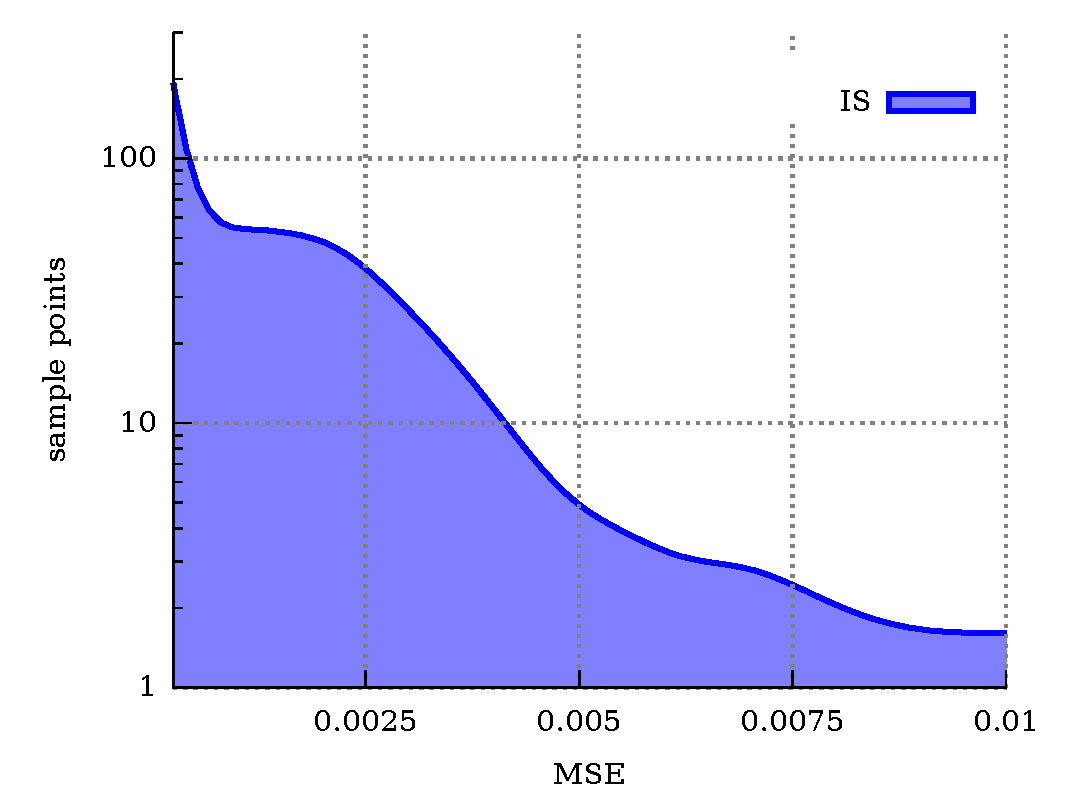
\includegraphics[width=.5\paperwidth]{graphics/mse_histogram_is_as1.pdf}}
      \myonly{2}{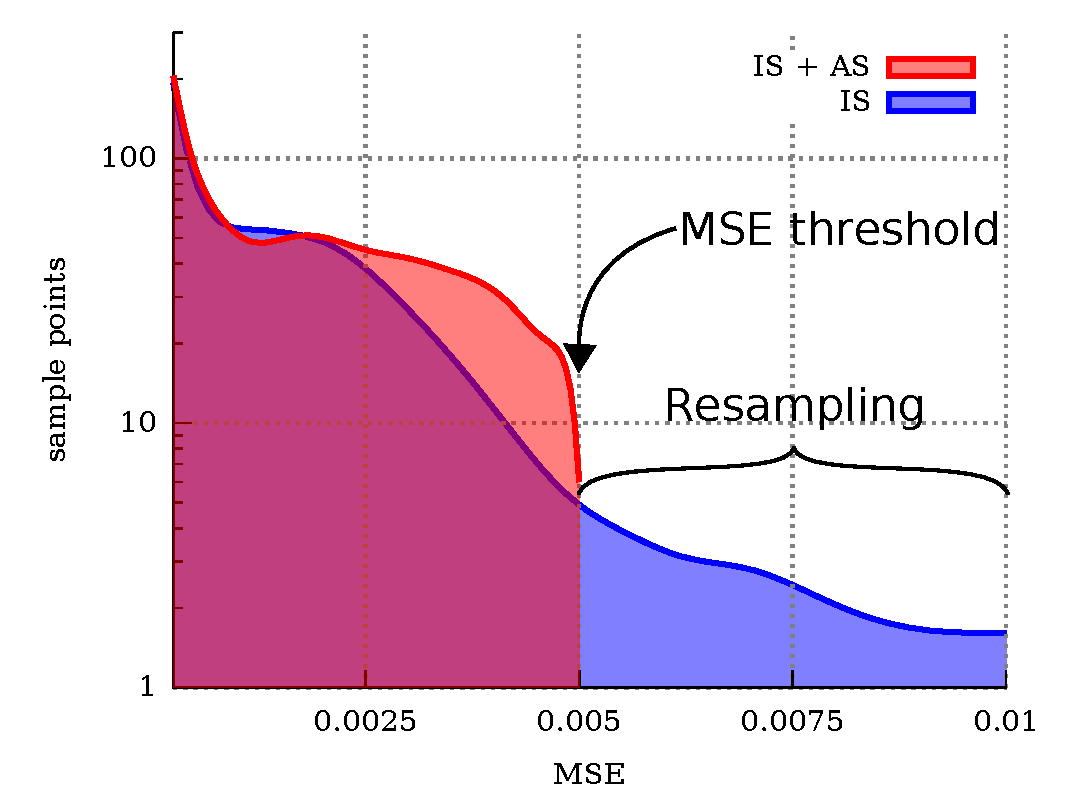
\includegraphics[width=.5\paperwidth]{graphics/mse_histogram_is_as2.pdf}}
      \begin{itemize}
        \myuncover{1}{2}{
        \item Even with importance sampling, high MSE peaks are possible
        }
        \myuncover{2}{2}{
        \item To reach a fixed MSE threshold, the number of rays for the sample point is increased
        }
      \end{itemize}
\end{frame}
